
\section{Introdução}

\begin{frame}
  \frametitle{Introdução}

  \textbf{Imagine o processo de discussão de ideias em uma rede:}

  \begin{alertblock}{}
    \vspace{5mm}

    \begin{itemize}
      \item Como modelar a influência de determinados agentes?
      \item Como se dá a percepção de informações ao longo do tempo?
      \item Como o surgimento de novas informações afeta essa dinâmica?
    \end{itemize}
    \vspace{5mm}

  \end{alertblock}
\end{frame}

\begin{frame}
  \frametitle{Introdução: Modelo Proposto}

  \textbf{Elaboramos um modelo onde:}

  \begin{alertblock}{}
    \vspace{5mm}

    \begin{itemize}
      \item Cada nó da rede tem um valor no intervalo contínuo de [-1, 1];
      \item Uma ligação $(i, j)$ significa que $i$ recebe informação de $j$;
      \vspace{5mm}

      \item A influência exercida por um nó é proporcional ao número de nós que
        recebem informação dele.
    \end{itemize}
    \vspace{5mm}

  \end{alertblock}
\end{frame}

\begin{frame}
  \frametitle{Introdução: Modelo Proposto}

  \textbf{Função discreta para influência $x$ e posicionamento perante
  uma informação $y$:}

  \begin{alertblock}{}

    \begin{equation}
      x_{t}(i) = y_{t}(i) \  l_{t}^{r}(i),
    \end{equation}

    \begin{equation}
      y_{t+1}(i) = \frac{\sum_{j} \  x_{t}(j)}{\sum_{j} \  l_{t}^{r}(j)},
    \end{equation}

  \end{alertblock}
  \vspace{5mm}

  onde $l_{t}^{r}(i)$ são as ligações do grafo reverso do nó $i$.
\end{frame}

\begin{frame}
  \frametitle{Introdução: Modelo Proposto}

  \textbf{Podemos concluir então que:}

  \begin{alertblock}{}
    \vspace{5mm}

    \textbf{\alert{O posicionamento de um nó $i$ perante uma informação} é a
      média das influências dos nós adjacentes ponderadas pelas suas ligações
      no grafo reverso.}
    \vspace{5mm}

    \textbf{\alert{A influência de um nó $i$} é seu posicionamento perante uma
      informação multiplicada por suas ligações no grafo reverso.}
    \vspace{5mm}

  \end{alertblock}
\end{frame}

\begin{frame}
  \frametitle{Introdução: Estudo de Caso}

  \begin{alertblock}{}
    \vspace{5mm}

    \textbf{\alert{Aplicamos a dinâmica proposta}} em rede publicada por Adamic e Glance
      \cite{Adamic:2005:PoliticalBlogs}.
    \vspace{5mm}

    \textbf{\alert{A rede}} consiste de blogs políticos (\textbf{nós}). Uma
      ligação entre um par $i, j$ corresponde a um \textbf{link} do blog $i$ para
      o blog $j$.
    \vspace{5mm}

    \textbf{\alert{Dados foram coletados em 2004, nos Estados Unidos}}, e
      correspondem à corrida presidencial entre George W. Bush e John Kerry.
    \vspace{5mm}

  \end{alertblock}
\end{frame}

\begin{frame}
  \frametitle{Introdução: Estudo de Caso}

  \begin{figure}
    \centering
    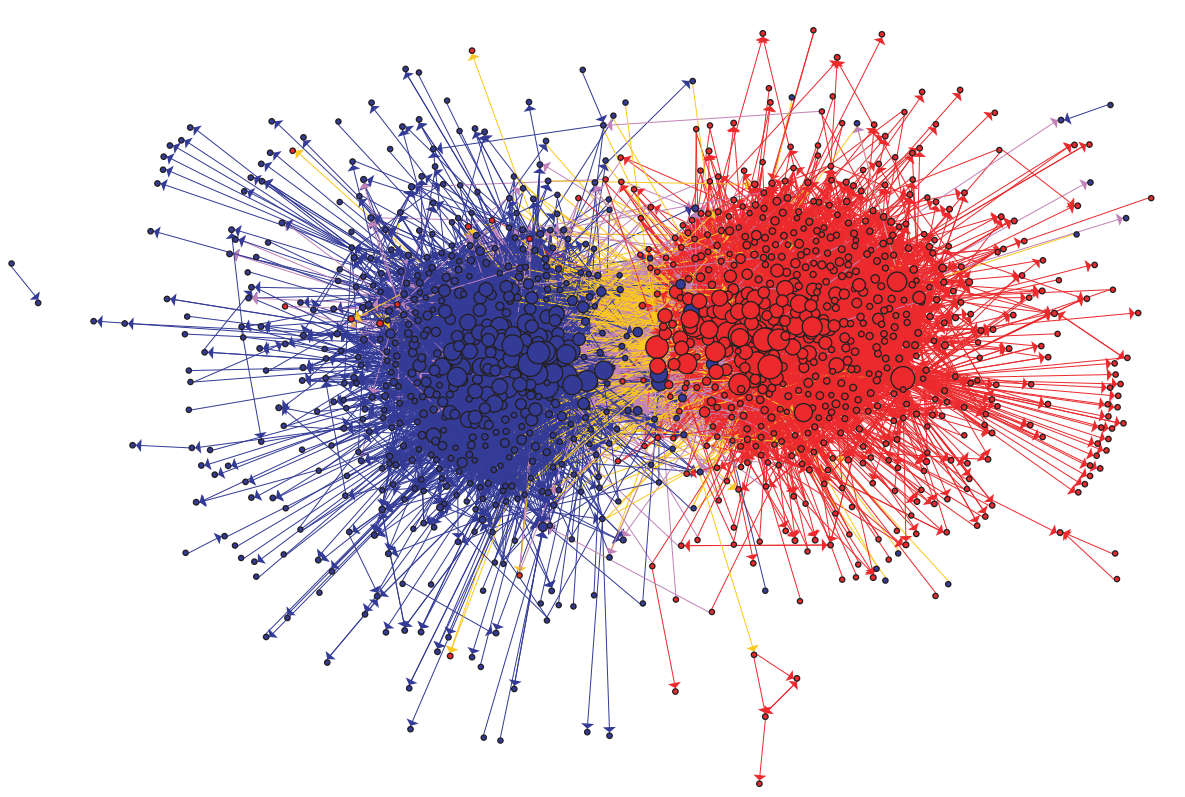
\includegraphics[scale=0.2125]{./figures/AdamicGlanceNetwork}
    \caption*{Rede de blogs políticos de Adamic e Glance
      \cite{Adamic:2005:PoliticalBlogs}: conservadores de vermelho, liberais de
      azul.}
  \end{figure}
\end{frame}

\begin{frame}
  \frametitle{Introdução: Estudo de Caso}

  \begin{figure}
    \centering
    \vspace{-10mm}
    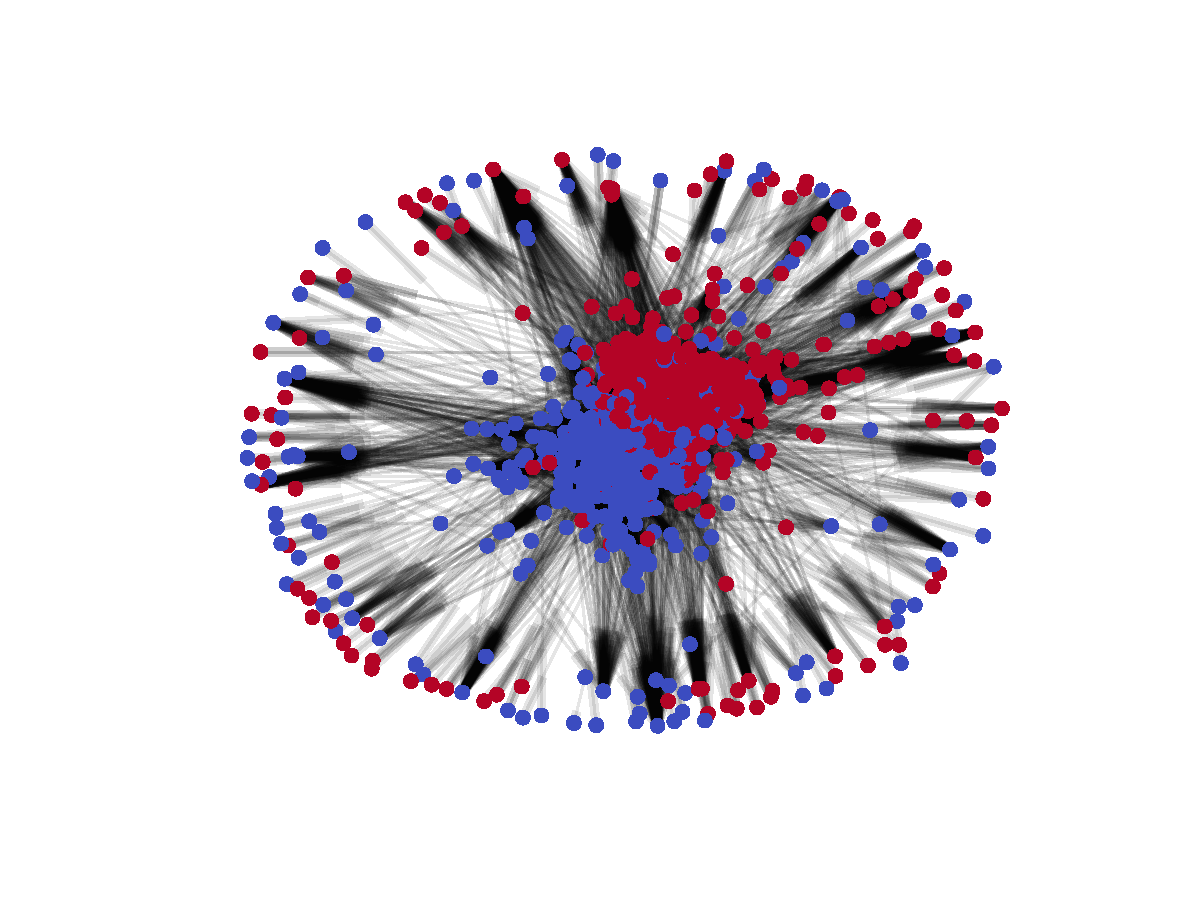
\includegraphics[scale=0.4]{./figures/99N000}
    \vspace{-5mm}
    \caption*{Rede anterior gerada no \texttt{Python}: conservadores de vermelho,
      liberais de azul.}
  \end{figure}
\end{frame}
